
\begin{figure}[h]
\centering

\includegraphics[width=0.5\textwidth]{res/intro/logo.png}
\end{figure}

\section{Company}
TSMW is a young company, which aims at the auto industry and provides own
software solutions together with chosen hardware that is available on the market
or provided by the customer, to build a system, supporting the car driver with a
specific task. If needed, the company provides an analysis and a preselection of
available hardware pieces, in terms of quality, availability and price to the
customer, as well as an objective recommendation.

The aims and objectives of the company are:

\begin{itemize}
  \item Development of support systems which satisfy the customer and the end
  user
  \item Creation of objectively fitting hardware selections for the customer 
  \item Long terms binding of the customer to the company, through good price
  and quality of the required system.
\end{itemize}

\section{Staff}
The following chapter introduces the TSMW team. The young company consists of 4
members which share the tasks between each other to achieve the most with the
given capacity, but also all have their special responsibility / role of their
own. Especially for a small company, it is of high importance to coordinate the
activities to meet the requirements of the customer.

\begin{table}[h]
\renewcommand\arraystretch{1}
\begin{tabular}{p{0.23\textwidth}p{0.23\textwidth}p{0.23\textwidth}p{0.23\textwidth}}
\begin{center}Markus\end{center} & 
\begin{center}Timo\end{center} & 
\begin{center}Simon\end{center} & 
\begin{center}Wojciech\end{center}
\\
\vspace{-1.2cm}\begin{center}Just\end{center} & 
\vspace{-1.2cm}\begin{center}Acquistapace\end{center} & 
\vspace{-1.2cm}\begin{center}Schneider\end{center} & 
\vspace{-1.2cm}\begin{center}Lesnianski\end{center}
\\
\vspace{-1cm}\begin{center}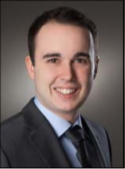
\includegraphics[width=0.2\textwidth]{res/intro/Markus.png}\end{center}
& 
\vspace{-1cm}\begin{center}
\includegraphics[width=0.2\textwidth]{res/intro/Timo.png}\end{center}
&
\vspace{-1cm}\begin{center}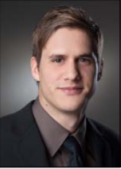
\includegraphics[width=0.2\textwidth]{res/intro/Simon.png}\end{center}
&
\vspace{-1cm}\begin{center}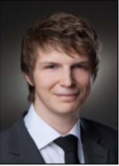
\includegraphics[width=0.2\textwidth]{res/intro/Ich.png}\end{center}
\\
\vspace{-1cm}\begin{center}Project Leader\end{center} & 
\vspace{-1cm}\begin{center}Software Architect\end{center} & 
\vspace{-1cm}\begin{center}Software Engineer\end{center} &
\vspace{-1cm}\begin{center}Designer \end{center}
\end{tabular}
\end{table}

To make the coordination of the activities possible, we require a clear
definition of roles and their interdependencies:

\subsection{Project Manager}
Project Manager is primary responsible for the communication with the customer
and acquisition of requirements, as well their transformation into tasks and
user stories. He supervises the development process and monitors the process
flow.

\subsection{Software Engineer}
The primary task of the Software Engineer is primary responsible for the
development of the system backend, decision making about the form of persistent
data and the advisement of the software architect. The Software Engineer creates
a selection of eligible hardware parts and together with the Project Manager,
presents them to the customer.

\subsection{Software Architect}
The main task of the Software Architect is the creation of the architecture, as
well as the consultation with all developers about the current development
decisions.

\subsection{Designer}
The Designer is responsible for the creation of a user interface prototypes, as
well as the development of the user interface throughout the development
process. He is also in charge of the company's corporate design and its logo.

\section{Product}
The requested system should be built into the customer's cars and support the
driver by bringing his car out of a parking position. Various sensors around the
car should provide safety during the process and the driver should always be
able to take control of the car. For the system, it should be of no matter,
weather the parking position is parallel or perpendicular. In further
development iterations, the process should also provide an external interface
for third party systems to start or stop a parking process. The system should be
capable of working with the traffic systems of all countries the customer's cars
are sold to and take into account the countries rules including the orientation
of the bidirectional traffic. For driver's convenience, the system should
provide a graphical interface with an overview over the current state of the
parking process, as well as the information received from the sensors.
